\subsubsection{\stid{2.10} PROTEAS-TUNE - Clacc: OpenACC in Clang and LLVM}\label{s:clacc}

\newcommand{\todo}[1]{\textbf{\textcolor{red}{#1}}}

\paragraph{Overview}

Heterogeneous and manycore processors (e.g., multicore CPUs, GPUs,
Xeon Phi, etc.) are becoming the de facto architectures for current
HPC platforms and future Exascale platforms.  These architectures are
drastically diverse in functionality, performance, programmability,
and scalability, significantly increasing the complexity that ECP app
developers face as they attempt to fully utilize available hardware.

A key enabling technology pursued as part of PROTEAS-TUNE is OpenACC.
While OpenMP has historically focused on shared-memory multi-core,
OpenACC was launched in 2010 as a portable programming model for
heterogeneous accelerators.  Championed by institutions like NVIDIA,
PGI, and ORNL, OpenACC has evolved into one of the most portable and
well recognized programming models for accelerators today.

Despite the importance of OpenACC, the only non-academic open-source OpenACC
compiler cited by the OpenACC website is GCC \cite{openaccOrgTools}.
However, GCC has lagged behind commercial compilers, such as PGI's, in
providing production-quality support for the latest OpenACC specifications
\cite{openACCValidationSuite}.  Moreover, GCC is known within the compiler
community to be challenging to extend and, especially within the DOE, is
losing favor to Clang and LLVM for new compiler research and development
efforts.

\textit{Clacc}~\cite{clacc:2018:denny} is a major component of the
PROTEAS-TUNE project.  Overall, the goal is to build on Clang and LLVM
to develop an open-source, production-quality OpenACC compiler
ecosystem that is easily extensible and that utilizes the latest
research in compiler technology.  Such an ecosystem is critical to the
successful acceleration of ECP applications using modern HPC hardware.
The PROTEAS-TUNE objectives for Clacc are:

\begin{enumerate}

\item Develop production-quality, standard-conforming OpenACC
compiler and runtime support as an extension of Clang and LLVM.  Two
compilation modes are being developed: (a) traditional mode, which
produces a binary, and (b) source-to-source mode, which produces
OpenMP source.

\item As part of the design, leverage the Clang ecosystem to enable
the future construction of source-level OpenACC tools, such as pretty
printers, analyzers, lint tools, debugger extensions, and editor
extensions.

\item Throughout development, actively contribute improvements to the
OpenACC specification, and actively contribute mutually beneficial
improvements to the upstream Clang and LLVM infrastructure.

\item As the work matures, contribute OpenACC support itself to
upstream Clang and LLVM so that it can be used by the broader HPC and
parallel programming communities.

\end{enumerate}

\paragraph{Key Challenges}

\begin{enumerate}

\item \textbf{OpenACC Support:} Developing production-quality,
standards-conforming OpenACC compiler and runtime support is a large
undertaking.  Complicating that undertaking further is the need for
optimization strategies that are competitive with existing commercial
compilers, such as PGI's, which have been developed over many years
since before the conception of the OpenACC standard.

\item \textbf{Source-to-Source:} Source-to-source translation to
OpenMP significantly reduces the effort to implement OpenACC and
offers additional capabilities, such OpenACC support for proprietary
OpenMP compilers.  However, a known issue with Clang is that its AST,
the source-level representation, was designed to be immutable.
Moreover, the AST represents the source after preprocessor expansions,
which harm readability and can prevent compilation with other
compilers.  Finally, sophisticated analyses and optimizations are
critical for lowering OpenACC's descriptive language to the more
prescriptive language of OpenMP, but these are best implemented at the
level of LLVM IR not the Clang AST.

\item \textbf{Production-Quality:} Clang and LLVM are sophisticated tools
with a complex codebase and a large team of developers who diligently screen
contributions to maintain a clean design and correct operation.  As for any
production-quality compiler, developing and contributing improvements to
Clang and LLVM can be significantly more challenging and time-consuming than
for research-quality compilers.

\item \textbf{OpenMP Alternative:} We believe that OpenACC's current
momentum as the go-to directive-based language for accelerators will
continue into the foreseeable future.  Nevertheless, some potential OpenACC
adopters hesitate over concerns that OpenACC will one day be replaced by
OpenMP features.  A tool to migrate OpenACC applications to OpenMP could
alleviate such concerns, encourage adoption of OpenACC, and thus advance
utilization of acceleration hardware in ECP applications.

\end{enumerate}

\paragraph{Solution Strategy}

~
\vspace{-1em}

\begin{tabular}{@{\hspace{-1.5em}}p{.6\textwidth}p{.4\textwidth}@{}}

\begin{enumerate}

\item A key Clacc design feature is lowering OpenACC to OpenMP.
Benefits include:

\begin{enumerate}

\item By building on Clang and LLVM's OpenMP support, it reduces the
effort necessary to construct a production-quality OpenACC
implementation.

\item It enables OpenACC support on OpenMP compilers other than Clang,
including proprietary compilers.

\item It facilitates repurposing existing OpenMP static analysis and
debugging tools for the sake of OpenACC.

\item It facilitates porting applications from OpenACC to OpenMP to
alleviate the aforementioned concerns about developing applications in
OpenACC.

\end{enumerate}

\end{enumerate}

&

\raisebox{-\totalheight}{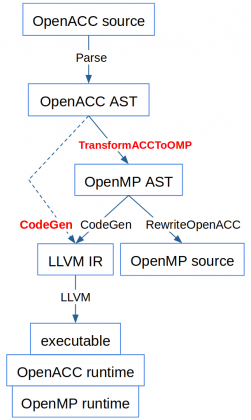
\includegraphics[scale=.3]{projects/2.3.2-Tools/2.3.2.10-PROTEAS-YTUNE/clacc.png}}

\end{tabular}

\vspace{-1em}

\begin{enumerate}

\setcounter{enumi}{2}

\item To handle Clang's immutable AST, Clacc's design includes a
TransformACCToOMP component that reuses a Clang feature called
TreeTransform, which was originally designed for C++ template
specializations.

\item To avoid preprocessor expansions in source-to-source mode, Clacc
includes a RewriteOpenACC component that reuses a Clang feature called
Rewrite.

\item To utilize LLVM IR analyses and optimizations, we are
investigating ongoing efforts toward a parallel LLVM IR.  Clacc could
use such an IR as a code generation target for OpenACC, either
directly or after translation to OpenMP extensions Clacc would
introduce to support OpenACC's descriptive features.

\item To stage our development effort, we are initially implementing
Clacc with two simplifications: we are implementing a prescriptive
OpenACC interpretation for correct behavior, and we are implementing
for C.  We will then extend Clacc with necessary analyses for a
descriptive interpretation and for C++.

\item To ensure Clacc's successful implementation and eventual acceptance
upstream, we continue design discussions with the Clang and LLVM
communities via mailing lists and other relevant forums.

\item Throughout Clacc development, we are continuously integrating the
latest upstream Clang and LLVM changes, and we are running and
extending the Clang and LLVM test suites to detect regressions and
incompatibilities.  We are also investigating OpenACC
benchmarks \cite{specAccel} and validation test
suites \cite{openACCValidationSuite} to ensure correct OpenACC
behavior and good performance.

\end{enumerate}


\paragraph{Recent Progress}

\begin{enumerate}
\item
  Extended Clacc to support additional features, including various
  OpenACC directives and clauses related to data motion and OpenACC
  Profiling Interface features motivated by integration with TAU.
\item
  Designed and prototyped various OpenMP extensions to support the
  above, including OMPT extensions.
\item
  Developed Gitlab CI config for x86\_64, ppc64le, and nvptx64,
  including a Summit node, on ORNL's ExCL cluster.
\item
  Performed preliminary GPU evaluation using SPEC ACCEL benchmarks.
\item
  Contributed numerous improvements to Clang and LLVM, including
  OpenMP and LLVM testing infrastructure improvements, and to the
  OpenACC specification.
\end{enumerate}


\paragraph{Next Steps}

\begin{enumerate}
\item
  Continue to implement Clacc support for critical OpenACC features
  based on the needs of ECP and other HPC apps and benchmarks, and
  pursue OpenACC optimizations and C++ support.
\item
  Continue contributions to upstream Clang and LLVM and to the OpenACC
  specification.
\end{enumerate}
